%\documentclass[margin=0mm]{standalone}
%\usepackage{tikz}
%\usepackage{pgfplots}
% \pgfplotsset{compat=newest}
%
%
%\usepackage{currfile,hyperxmp}
%\usetikzlibrary{math,matrix,fit,positioning}
%\usepgfplotslibrary{groupplots}
%
%
%\begin{document}

  

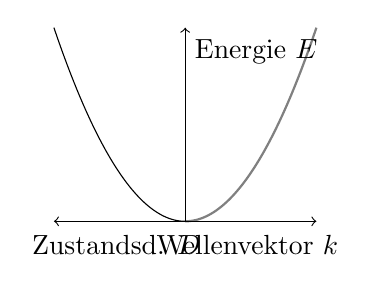
\begin{tikzpicture}
%\useasboundingbox (-1.0,-1.0) rectangle (10.2,4.2);
%\draw (-1,-1.0) rectangle (10.2,4.2);
%

 
\begin{axis}[
    height=3cm,
    width=4cm,
    xtick pos = bottom,
    scale only axis,
            separate axis lines,
  axis x line=none,
  axis x line shift=0pt,
  %xlabel shift=10pt,
  axis y line=none,
  axis y line shift=0pt,
%  ylabel shift=10pt      
 % axis y line=left, clip=true,
  ymin = -5.5, ymax = 25,
%  ytick = \empty,
%  xtick = {-3,-2, -1, 0,1,2,3},
%,ytick pos = left, ytick = {0}, 
% xmin=1320, xmax = 1520, xtick = {1415}, xticklabel = {1415}
 %ylabel = {Energie $E$}, % xlabel = {Wellenvektor $k$},
 ytick = \empty, yticklabel = \empty,
 xtick = \empty, xticklabel = \empty,
 %xtick = {0, 10},
 %xticklabels = {0, $E_F$},
%ylabel = {extinktion}, xlabel = {energy (eV)},
%ytick pos = left, 
% xmin=-5, xmax = 5,
 ]
\
%\addplot[blue,thick, domain= -4:-8, samples=100]{ 1/ (exp(x) + 1)  - 0.15* exp(- (x+6)^2 / 0.25) };
%\addplot[blue, thick,domain= 4:8, samples=100]{   1/ (exp(x) + 1)  +  0.15* exp(- (x-6)^2 / 0.25)) };
\addplot[ gray, thick, domain=0:5, samples=100]{x^2};
\addplot[ black, thin, domain=-5:0, samples=100]{x^2};

\draw[<->] (-5, 0) node[right, yshift=-3mm,xshift=-4mm] {Zustandsd. $D$} -- (5,0) node[left, yshift=-3mm,xshift=+4mm] {Wellenvektor $k$};
\draw[->] (0,0) -- (0,25) node[right,yshift=-3mm] {Energie $E$};

%\addplot[red, thick,domain=0:16, samples=100]{sqrt(x) / (exp((x-10)/1) + 1)};

%\draw[|-|,red] (9, 1.6) -- (11, 1.6) node[right] {\footnotesize $2 k_B T_{hot}$};
%\draw[|-|] (-2, 0.4) -- (2, 0.4) node[right] {\footnotesize $k_B T_{hot}$};

%\draw[|-|] (-6, -0.03) node[left] {\footnotesize $h \nu$} -- (6, -0.03) ;

\end{axis}


\end{tikzpicture}

%\end{document}